\documentclass[12pt,letterpaper]{article}
\usepackage[utf8]{inputenc}
\usepackage[margin=1in]{geometry}
\usepackage[english]{babel}
\usepackage{booktabs}
\usepackage{graphicx}
\usepackage[table,xcdraw]{xcolor}
\usepackage{appendix}
\usepackage{indentfirst}
%\usepackage[backend=biber,natbib=true,doi=true,citestyle=apa]{biblatex}
\usepackage{multirow}
\usepackage{xassoccnt}
\usepackage{blindtext}
\usepackage{setspace}
\usepackage{longtable}
\usepackage{todonotes}
\usepackage{quoting}
\usepackage{fancyhdr}
\usepackage{verbatim}
\usepackage{lipsum}
\usepackage{epigraph}
\usepackage{url}

\setlength{\epigraphwidth}{0.35\linewidth}
\setlength{\epigraphrule}{0pt}
\renewcommand*{\textflush}{flushright}
\renewcommand*{\epigraphsize}{\normalsize\itshape}
\newcommand*{\myquotingsource}{}
\newenvironment{myquoting}[1]{%
  \renewcommand*{\myquotingsource}{#1}
  \begin{quoting}[font={itshape},leftmargin=3em,rightmargin=3em]%
}{%
  \par\medskip
  \myquotingsource
  \end{quoting}%
}
\renewcommand{\baselinestretch}{1.6} 
\newcounter{todocounter}
\newboolean{showComments} 
\setboolean{showComments}{true}
\newcommand{\customComment}[3]
{\stepcounter{todocounter}
  \ifthenelse{\boolean{showComments}}{\todo[color=#2,inline]{#1 \thetodocounter: #3}}{}
}
\newcommand{\jm}[1]{{\color{red}#1}}
\newcommand{\jen}[1]{{\color{red}#1}}
\newcommand{\ac}[1]{{\color{red}#1}}

\pagestyle{fancy}

\bibliography{references}


\title{Tactile Map Tiles: Improving Navigational Access for Deaf-Blind Individuals Using Custom 3D-Printed Maps}
\author{Anat Caspi and Jennifer Mankoff}
\date{January 2019}

\begin{document}

\maketitle
\thispagestyle{empty}

\tableofcontents
\clearpage
\section*{Abstract}
{
\setstretch{1.2}

\normalsize
Mankoff and Caspi, in \textbf{partnership} with the Taskar Center for Assistive Technology \todo{or AccessMaps?} (which Caspi runs)\todo{XX other partners}, and key stakeholders will, in the course of this three year project, create a navigation solution for Deaf-Blind individuals to easily create custom tangible maps that meet their diverse needs. \todo{Should we also mention soundscape?}.
The \textbf{goal} of this project is to improve the navigation services available to Deaf-Blind individuals and give them the independent ability to create their own maps.  The \textbf{objectives} are: 1) to extend the AccessMaps interface to support need and route specification; 2) to automatically optimize map design based on specific needs; 3) to connect map production to existing online printing services. Anticipated \textbf{outcomes} include: 1) Deaf-Blind individuals and those who support them will have the ability to independently create custom maps; 2) Custom maps will improve the navigation experience of Deaf-Blind individuals; 3) Cost and time needed will not exceed existing services; 4) The solution will be integrated into the existing AccessMaps infrastructure. The expected products are an algorithm for creating custom maps, an accessible interface for specifying customization parameters, and software integration with AccessMaps. 
}

\clearpage
\pagenumbering{arabic} 

%\section{Rules}
%Comment out this section for the proposal submission.
%\begin{itemize}
    \item The page limit for this entire document is 50 pages. However the table of countents and abstract don't count toward that limit. You can separate them from the pdf once you generate it and (I think) you upload them seperately.
    \item The budget should be 195,000 to 200,000. A budget narrative / justification should be provided as a separate document that does not count toward your page limit. 
    \item The time limit is 36 months
    \item Vitae of staff or consultants should (I think) be uploaded separately and should include information that is specifically pertinent to this proposed project. If collaboration with another organization is involved in the proposed activity, the application should include assurances of participation by other parties, including written agreements or assurances of cooperation.
    \item Figure out what stage you are aiming at. If you are writing a development proposal:
    \begin{description}
    \item[Proof of concept] means the stage of development where key technical challenges are resolved. Stage activities may include recruiting study participants, verifying product requirements, implementing and testing (typically in controlled contexts) key concepts, components, or systems, and resolving technological challenges. A technology transfer plan is typically developed and transfer partner(s) identified, and plan implementation may have started. Stage results establish that a product concept is feasible.
    \item[Proof of product] means the stage of development where a fully-integrated and working prototype, meeting critical technical requirements, is created. Stage activities may include recruiting study participants, implementing and iteratively refining the prototype, testing the prototype in natural or less-controlled contexts, and verifying that all technical requirements are met. A technology transfer plan is typically ongoing in collaboration with the transfer partner(s). Stage results establish that a product embodiment is realizable.
    \item[ Proof of adoption ] means the stage of development where a product is substantially adopted by its target population and used for its intended purpose. Stage activities typically include completing product refinements and continued implementation of the technology transfer plan in collaboration with transfer partners. Other activities include measuring users’ awareness of the product, opinion of the product, decisions to adopt, use, and retain products; and identifying barriers and facilitators impacting product adoption. Stage results establish that a product is beneficial.
    Exploration and discovery means the stage of research that generates hypotheses or theories through new and refined analyses of data, producing observational findings and creating other sources of research-based information. This research stage may include identifying or describing the barriers to and facilitators of improved outcomes of individuals with disabilities, as well as identifying or describing existing practices, programs, or policies that are associated with important aspects of the lives of individuals with disabilities. Results achieved under this stage of research may inform the development of interventions or lead to evaluations of interventions or policies. The results of the exploration and discovery stage of research may also be used to inform decisions or priorities;
        \end{description}
  \item If you are writing a research proposal,
  \begin{description}
   \item[Intervention development] means the stage of research that focuses on generating and testing interventions that have the potential to improve outcomes for individuals with disabilities. Intervention development involves determining the active components of possible interventions, developing measures that would be required to illustrate outcomes, specifying target populations, conducting field tests, and assessing the feasibility of conducting a well-designed
intervention study. Results from this stage of research may be used to inform the design of a study to test the efficacy of an intervention;
   \item[ Intervention efficacy] means the stage of research during which a project evaluates and tests whether an intervention is feasible, practical, and has the potential to yield positive outcomes for individuals with disabilities. Efficacy research may assess the strength of the relationships between an intervention and outcomes, and may identify factors or individual characteristics that affect the relationship between the intervention and outcomes. Efficacy research can inform decisions about whether there is sufficient evidence to support “scaling-up” an intervention to other sites and contexts. This stage of research may include assessing the training needed for wide-scale implementation of the intervention, and approaches to evaluation of the intervention in real-world applications; and
  \item[ Scale-up evaluation] means the stage of research during which a project analyzes whether an intervention is effective in producing improved outcomes for individuals with disabilities when implemented in a real-world setting. During this stage of research, a project tests the outcomes of an evidence-based intervention in different settings. The project examines the challenges to successful replication of the intervention, and the circumstances and activities that contribute to successful adoption of the intervention in real-world settings. This stage of research may also include well-designed studies of an intervention that has been widely adopted in practice, but
  2 of 34
lacks a sufficient evidence base to demonstrate its effectiveness.
    \end{description}
\end{itemize}
%\section{Criteria}
%Comment out this section for the proposal submission.
%n\begin{description}
\item[For Research:] A research project that will generate findings that can be used to maximize the full inclusion and integration into society, employment, independent living, family support, or economic and social self-sufficiency of individuals with disabilities, especially individuals with the most severe disabilities.
\item[For Development:] A development project that will generate a product or products (e.g., materials, devices, systems, methods, measures, techniques, tools, prototypes, processes, or intervention protocols) that can be used to maximize the full inclusion and integration into society, employment, independent living, family support, or economic and social self-sufficiency of individuals with disabilities, especially individuals with the most severe disabilities.
\end{description}

\subsection{Scoring}
Applications are scored by assigning a maximum of 100 points across five criteria. 

\begin{itemize}
    \item Importance of the problem (20 points). The Director considers the importance of the problem.
    \begin{itemize}
\item  The extent to which the applicant clearly describes the need and target population.
\item The extent to which the proposed activities further the purposes of the Act.
\item  The extent to which the proposed project will have beneficial impact on the target population.
    \end{itemize}
    \item Design of development activities (50 points). Development proposals only. The Director considers the extent to which the design of development activities is likely to be effective in accomplishing the objectives of the project, including: 
    \begin{itemize}
\item The proposed project shows awareness of the state-of-the-art for current, related products. 
\item The proposed project employs appropriate concepts, components, or systems to develop the new or improved product.
\item  The proposed project employs appropriate samples in tests, trials, and other development activities.
\item The proposed project conducts development activities in appropriate environment(s).
\item Input from individuals with disabilities and other key stakeholders is obtained to establish and guide proposed development activities.
\item The applicant identifies and justifies the stage(s) of development for the proposed project; and activities associated with each stage.
    \end{itemize}
\item Design of research activities (50 points) (research proposals only). The Director considers the extent to which the design of research activities is likely to be effective in accomplishing the objectives of the project. Specifically, the extent to which the methodology of each proposed research activity is meritorious is important.
\begin{itemize}
    \item The proposed design includes a comprehensive and informed review of the current literature, demonstrating knowledge of the state-of-the-art.
    \item Each research hypothesis or research question, as appropriate, is theoretically sound and based on current knowledge.
    \item Each sample is drawn from an appropriate, specified population and is of sufficient size to address the proposed hypotheses or research questions, as appropriate, and to support the proposed data analysis methods.
    \item The source or sources of the data and the data collection methods are appropriate to address the proposed hypotheses or research questions and to support the proposed data analysis methods.
    \item The data analysis methods are appropriate.
    \item Input of individuals with disabilities and other key stakeholders is used to shape the proposed research activities.
    \item The applicant identifies and justifies the stage of research being proposed and the research methods associated with the stage.
\end{itemize}
    \item Plan of evaluation (5 points)
    \begin{itemize}
\item The extent to which the plan of evaluation provides for periodic assessment of progress toward implementing the plan of operation.
\item The extent to which the plan of evaluation will be used to improve the performance of the project through the feedback generated by its periodic assessments.
    \end{itemize}
    \item Project staff (15 points)
    \begin{itemize}
\item In determining the quality of the project staff, the Director considers the extent to which the applicant encourages applications for employment from persons who are members of groups that have traditionally been underrepresented based on race, color, national origin, gender, age, or disability.
\item In addition, the Director considers the extent to which the key personnel and other key staff
have appropriate training and experience in disciplines required to conduct all proposed activities.
    \end{itemize}
    \item Adequacy and accessibility of resources (10 points). The Director considers the adequacy and accessibility of the applicant's resources to implement the proposed project.
    \begin{itemize}
\item The extent to which the applicant is committed to provide adequate facilities, equipment, other resources, including administrative support, and laboratories, if appropriate.
\item The extent to which the facilities, equipment, and other resources are appropriately accessible to individuals with disabilities who may use the facilities, equipment, and other resources of the project.

    \end{itemize}
\end{itemize}
\section{Introduction and Problem Definition}



%SK:  copied this text from source sited below. Can we plug it in to the very beginning of the proposal as an italicized/centered quote?
\begin{myquoting}{\cite{jaiswal2018participation}}

Deafblindness, also known as dual sensory loss, is a varying combination of visual and
hearing impairment in the same individual. Interest in this topic has increased recently due
to evidence suggesting an increase in prevalence of this condition among older adults. Persons with deafblindness frequently experience participation barriers and social isolation. Developing an understanding of their experiences can inform the design of programs and
policies to enhance participation of people with deafblindness in society .
\end{myquoting}

Individuals who are Deaf-blind represent a small percentage of the US population, but one with highly specialized transportation and navigational needs that are to date unmet. No current technology or apps communicate information about the layout of an environment in a manner that is easily and portably consumable by this cohort. Our proposal seeks to close this information gap and enable this community to create its own maps rather than rely on a mediator to decide what information is relevant to them. By doing so, we hope to lower or remove transportation barriers that prevent Deaf-blind persons from participating fully in society. 

\subsection{Problem: A Fundamental Communication Barrier With Significant Quality of Life Implications}

Maps are an important tool for navigation because they help people to understand the spatial layout of an environment. However, they are inherently visual and content-rich. One solution that has a long history in the Blind and Deaf-blind community is tactile maps – maps that use raised features to represent spatial layouts and landmarks. Common approaches include embossing, printing in Braille, and “swell” (microcapsule) paper. These approaches can be used to create a two-layer tactile visualization from an image (\textit{e.g.}, \cite{miele2006talking}).

However, maps created by these approaches suffer from some serious limitations. First, they can be very costly \cite{rice2005design}, are non-scalable, and the technology for creating them is not readily available. Second, they lack standardization as they are largely a reflection of work put forth by Orientation and Mobility specialists who do not envisage the work as traditional cartographers would \cite{lobben2012tactile, gual2012visual}. Third, they represent limited types of information because they lack the expressive range of a solution that can vary more in height; for example, one cannot represent elevation changes and finer grained qualities of pavements without explicitly writing them into the map. Further, feature density and selecting the map scale creates a significant problem in the physical manifestation of a map due to the minimum size required for a finger to sense a tactile feature. Finally, in the past, reliable stewards who were skilled in creating tactile maps chose the features they deemed important on the users’ behalf; this resulted in limited customizability and a complete lack of user agency in determining the type and amount of information available on the map. 


More recently, digital cartographic solutions are replacing all other maps. These solutions have the important advantage of being maintainable with relevant updated information about changing street environments and transit services. However, personalized navigational mobile apps, such as Directions on Google Maps \cite{GoogleMaps}, are fundamentally visual and generally exclude blind, low vision and Deaf-blind populations. Common solutions are Blind-Aware phone applications targeting Blind navigators, which are GPS programs that provide auditory turn-by-turn directions (but little information that allows for exploration). To use these apps, Deaf-blind people must translate auditory prompts to tactile messages via Braille displays; this way of consuming the auditory information from these apps has a significant usability drawback: Braille displays refresh slower than spoken content, and therefore the apps' auditory cues, which are often verbose and generated at a fast pace, are difficult to comprehend for users with a Braille display interface.  

In light of the preceding constraints and limitations of both digital and tactile paper approaches, to solve this critical communication problem, our solution has to meet the following six \textbf{design criteria}: 
\begin{itemize}
 \item The solution must be scalable, reproducible, and cost effective. 
 \item The solution must use best available pedestrian-centered information and standard tactile symbols. 
 \item The solution must improved expressivity of tactile maps, enabling more information to be included in the same spatially compact touch real estate.
 \item The solution must be customizable to user-specified parameters (including purpose of travel, area of interest, and other user-specific travel preferences). 
 \item The solution must be provided in a simple, open interface, allowing users of all abilities to create and customize their own maps. 
 \item The solution must contain current mapping data, and be updatable or provide a way for Deaf-blind users to be made aware of changes to the landscape in the mapped region.
\end{itemize}
Significantly, our solution must address usability criteria pertaining to the user experience of interacting with both our interfaces and maps. 

Based on these criteria, our solution will focus on creating a human-centered smart toolset and a cost-effective service system that allows Deaf-blind users to produce customized, 3D printed tangible maps on their own. %We will use 3D printing to reduce costs and extend reach and scalability of tactile maps. 
Specifically, in our development project, we will address each criterion with the following \textbf{development activities}:

\begin{itemize}
    \item We will extend our aggregated accessibility map codebase to support a production-level pipeline that produces 3D printed map models thereby extending reach and scalability (while reducing costs) of tactile maps.  (Section \ref{sec:fabrication})
    \item We will use the OpenSidewalks pedestrian-centric data standard \cite{bolten2017} and standard tactile symbols (\cite{BANA}) to represent features in a replicable, pedestrian-appropriate manner.  (Section \ref{sec:mapping-data})
    \item We will use multi-variable optimization algorithms to balance information richness with tactile usability (to enable appropriate use and density of tactile real estate). (Section \ref{sec:optimize})
    \item We will use a parameterized cost function to accommodate the user’s custom requirements about the area of travel, type of travel, and user needs and preferences.  (Section \ref{sec:parameters})
    \item We will focus on building accessible, user-tested and user-friendly interfaces that are integrated into our production-level accessible map, designing all exchanges to be easily navigable using a 14 cell portable Braille reader (the most constrained interface we know to be in use). (Section \ref{sec:accessmap-integration})
    \item We will create optional services that will let users: (1) have their model printed and sent to them (at cost), and (2) subscribe to email alerts regarding any changes to the mapped region in the digital map repositories. (Section \ref{sec:alerts})
\end{itemize}

Our solution combines simple, accessible interfaces with complex data integration and smart routing. To our users, the entire solution will be seamlessly presented in a workflow through which Deaf-blind pedestrians access a website, select the area of travel, the type of travel they wish to undertake in the area, and travel preferences. They are given the opportunity to verify the map location and features via non-visual, text-based exchange before downloading it for a specified duration or choosing to print the map. The entire exchange is enabled and specifically designed for a portable 14-cell Braille display. At the conclusion of the interaction, users can decide whether to subscribe to email alerts to keep their tactile maps current and serviceable. 

%SK paragraph
In sum, we intend to produce three main \textbf{project deliverables}: an accessible web interface that lets users customize and create their own maps; an algorithm for creating custom tactile maps that is seamlessly integrated into a current accessible map solution; and an email notification system informing users about changes to landscape and service modifications in a specified travel area. Using our tools, Deaf-blind pedestrians will finally be able to access current, relevant, pedestrian-centric digital map and transit information. By doing so, they will become stronger decision makers, more self-reliant travelers, and less socially isolated members of society.

\begin{comment}
In sum, we have three main \textbf{project deliverables}:
\begin{itemize}
    \item An \textit{accessible web interface }that lets users customize and create their own maps
\item An \textit{algorithm for creating custom tactile maps} that is seamlessly integrated into a current accessible map solution.
\item An \textit{email notification system} informing users about changes to landscape and service modifications in a specified travel area.
\end{itemize}
Using our tools, Deaf-blind pedestrians will finally be able to access current, relevant, pedestrian-centric digital map and transit information. By doing so, they will become stronger decision makers, more self-reliant travelers, and less socially isolated members of society. 
\end{comment}

\subsection{Population: Who is being impacted}
%Digital mapping technology has made a transformative difference in the manner people, particularly urban residents, tackle their daily navigational needs; many people use smart phones and mapping applications to plan trips using the most up-to-date information to ensure they get to their destinations quickly and safely. 
More than 160 million blind, low-vision, and deaf-blind people worldwide have not realized the full potential of digital maps. 
%People in these groups often use special-purpose portable devices to solve specific map accessibility problems, such as finding location information via an external GPS device, and accessing printed text using optical character recognition (OCR).
Our primary focus will be on Deaf-blind individuals. Although few estimates of the global deaf-blind population exist, the population in the United States alone is believed to be at least 50,000 
(comprising of about 10,000 children and 43,000 adults) \cite{NCDB} and likely much larger because many in this
population identify with only their dominant impairment. For example, the Board of Directors of the National Association of Regulatory Utility Commissioners, convened in 2008, estimated between 70-100,000 of their consumers are Deaf-blind \cite{NARUC}.
%About 35-40,000 Americans are Deaf-blind \cite{watson1993model}, and 
Prevalence is higher among the elderly population, and with this demographic increasing, so has the population of Deaf-blind in the U.S. been increasing. This group's needs are often not considered in the design of technology, which may be accessible to blind, or Deaf persons, but not both. 

Although our focus is on Deaf-blind, it is worth noting that tactile maps are also of great interest for the Blind, and indeed the National Federation for the Blind has published a report on tactile graphics \cite{lobben2015tactile}. 3\% of Americans are legally blind (3.4 million people); vision loss is among the top 10 disabilities.
Thus our work will have impact both on an important and understudied smaller group (Deaf-blind) and also serve the needs of a much larger group. 


\subsection{Importance: Significant Unmet Barrier}

% Trying to drive home that there's no other option (tactile iPads aren't here yet and additive manufacturing is growing everywhere.
% Also drive home how dire the current situation is
For people who are Deaf-blind, unmet transportation needs pose a major barrier to accessing every facet of social participation, including access to on-location employment, healthcare resources, education, financial resources and community participation. 
Among these, participation in the workforce is one of the most important because of its ongoing impact on financial independence and social inclusion, and it is particularly limited for Deaf individuals and Blind individuals \cite{zwerling2002workforce}.  
In 2012, half of the individuals with a disability who were not working reported ``Lack of transportation'' as the third greatest barrier to work, following only ``one's own disability'' and ``lacking training'' \cite{BLS}.
Workforce inclusion aside, a lack of mobility has been generally linked to social exclusion \cite{kenyon2002transport}.


% AC: do we need to explain why social exclusion is a problem?

Trip planning (whether for navigating to a specific destination, for taking a multi-modal trip or for exploration) is a critical link in the complete door-to-door trip \cite{AttriCompleteTrip}, and is especially important to people who are Deaf-Blind, for whom minute changes even on a well-practiced route may completely subvert a trip.  Lack of reliable, current, sufficiently detailed information about transportation networks and pedestrian routing constitute a major part of the mobility problem for all people with special travel needs. However, efforts to ameliorate this problem today are largely focused around improving and building out the digital cartography infrastructure where the visual or audio experience of maps ranks above all senses. The concerns is that all the emerging data-driven, dynamic and engaging forms of mapping being produced today provide exclusively audio-visual articulations of the environment, thereby excluding Deaf-blind individuals and further hindering the downstream development of services and applications that could address the transportation needs of this cohort. 

There is data-supported recognition that this problem requires attention.
The Accessible Transportation Technology Research Initiative (ATTRI) studied the transportation challenges of people with all types of disabilities and identified significant unmet barriers to using transit, user needs when taking transit, and the most common issues with technology.
Of the three running examples of needed assistive technology solutions to address barriers associated with access to information, two were 
``tactile navigation/information device for individuals who are deaf-blind'' and ``proximity-based public announcements through text-based messaging'' alerting people about current conditions on the ground. Our work proposes a solution to address both.

In sum,  aids that meet the trip planning and navigational needs of Deaf-blind individuals are limited, and by our estimation, few are under development.
Thus, we must consider how experiences for people with both vision and hearing loss can be sensitively designed to provide comfortable, safe and delightful experiences mediating both destination-directed travel and exploration of the urban environment. 



\subsection{Broader Impact}
We believe this development project could benefit downstream creation of other products for individuals with disabilities.
The Tactile Map Tile application will be built using relatively inexpensive and scalable technology and open data sets (e.g., transit data APIs, OpenSidewalks data, and OpenStreetMap infrastructure), and could therefore be used and consumed in other applications. 
This data and tools can benefit municipalities and transit agencies by helping shift passengers with disabilities onto fixed‐route transit. 
Because ADA paratransit is 7‐to‐10 times more expensive per passenger trip than fixed route transit \ac{(citation)}, any shift in passenger travel from paratransit to fixed‐route transit helps transit agencies control and potentially reduce operating and capital costs associated with
operating paratransit service. 
Upon completion, our application source code will be available using existing standards in open‐source development.
Tactile Map Tile will provide an affordable, reproducible, informative map artifact and the outcomes of this project will result in beneficial lessons, methodologies and tools that can be applied by transportation service providers in many regions, helping to attract and retain new travelers with and without disabilities.


\subsection{Preliminary Development: Proof of Concept Elucidated Needs of Mitigating Daily Exclusion}
\label{sec:pilot}

\ac{the outcomes of this section are:
(1) explain that we have deep reach into this community already. 27 DB in this area out of the known 40 adults in Seattle, is pretty huge.
(2) that we were able to assess needs with the population and one of the outcomes was identifying the information types that we need to map for them, including everything that is found in the mapping-data section.
(3) that we found participants needed solutions to enable greater independence in navigation, wayfinding and exploration.
(4) that participants needed to be kept up to date on changes in their environment because they won't just be able to see it.
(5) that success will really depend on how well we integrate what we provide with the devices they already have, and the most limiting one is a 14 cell Braille reader so we should design for that. The Ladner study also supports this.
}

Pairing a participatory, data-driven design approach together with interdisciplinary collaboration, we previously created 3D printed, parametrically designed maps to elicit feedback from Orientation and Mobility Specialists and would-be users who are Deaf-blind.


\begin{figure}
    \centering
    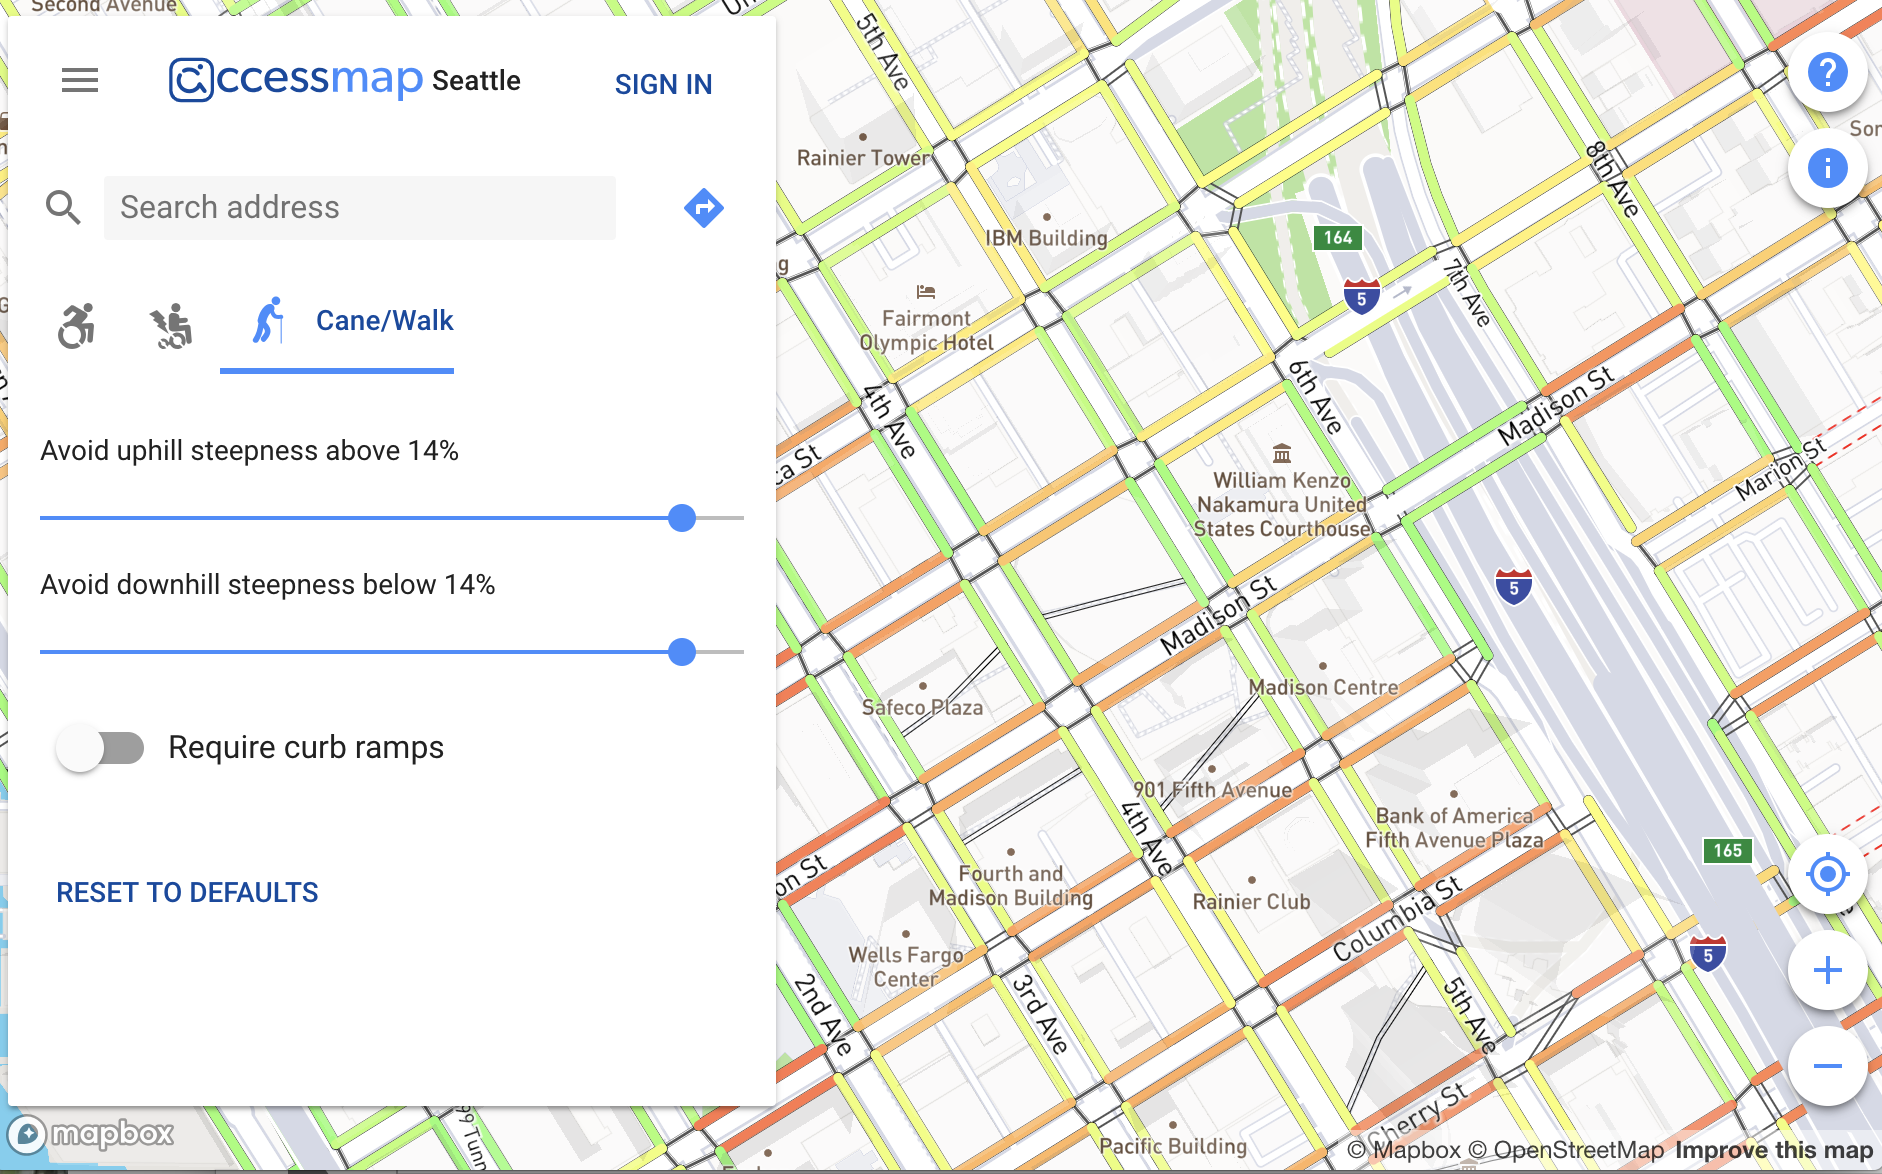
\includegraphics[width=5in]{pics/accessmap.png}
    \caption{Tactile Maps Generated Via Preliminary Study}
    \label{fig:pilot}
\end{figure}


The map tiles were produced for two areas in Seattle that would be familiar to our users. The map was scaled such that 1”=200’ (1mm=2.4m).  This scale accommodated an area roughly 3x4 blocks.   
Due to 3D print bed constraints, map tiles were limited to ~8” x 5.5”. In order to capture an area that includes both the forthcoming Judkins Park Transit Station, and Seattle Lighthouse for the Blind at this scale 3 tiles were needed.   

Based on preliminary feedback from expert users, basic features of the urban pedestrian environment were legible at this scale.  Further usability testing and symbol development must be conducted in order to confidently say if this scale is appropriate as a navigational aid.   The case study map series was printed with slight variation in symbol style, and size on each tile in anticipation of user testing, however it seems likely that the variations produced were not adequately different and should be exaggerated more for future testing.

Appendix C map features printed with measurements.
Experts interviewed indicated a more detailed tactile representation of smaller sites might also be valuable.  Potential areas cited that would benefit from the availability of detailed maps include transit stations, and complex intersections, particularly non-perpendicular intersections and those involving the junction of three or more streets.  Additional interviews or a survey distributed more broadly would be useful in identifying other areas of interest, and what features of these spaces should be prioritized for representation.  

There is an additional opportunity to apply the approach used in this project to developing maps that convey different types of information.  Zoomed way out, it would be relatively easy to create maps that are more reflective of the broader context of an area or district.  Here again there is an opportunity to create a basic symbol set for features that would be desirable in order to better understand how an area is situated in place.  In addition to the standard cartographic information such as scale and cardinal direction, this may include green spaces, water bodies, arterials, district lines, etc.  


We conducted a  preliminary study in a focus group meeting of 27 Deaf-blind individuals to assess need. We asked participants to explain how they travel and the issues most troublesome to them. 
Our study aimed to better understand how Deaf-blind people currently access community travel and 
accommodate inaccessibility in the built environment. In addition we were interested to know whether a tangible map we 3D printed for the area in which the participants met us added to their overall knowledge and confidence about traveling in that neighborhood.


%We first asked the participants to meet us at the public library where the Deaf-blind Service Center organizes community events. 
%We observed their arrival to the library location. 
Of the participants in the focus group, four individuals agreed to participate in semi-structured interviews at a public library location familiar to them. We asked about their travel habits and strategies for using inaccessible built environments.
We presented the participants a tactile map of the area in which we met them and asked participants to survey the tactile map. We asked them to find the location of the library in which we met, which was signified by a \textit{landmark} tactile icon. \jm{xx ANAT: do we have a picture of this?} We asked participants to explore the area and note any items, landmarks, street-names, buildings, bus stops or features that they understood to be in the area their hands were exploring. %We observed the manner in which they explored the map and recorded their exploration via video. %It should be noted that since individuals were conversing 
Participants conversed with us through  interpreted sign language, and the whole session was video recorded. %, they would interrupt the exploration session to explain to us what they understood about the map.

%We extracted the following key insights, which we will use to inform the design of this development project and we will also factor directly into the production of parsimonious yet useful tactile representations on the maps:

\textbf{“I don’t see anything and I feel limited in independence. I walk the same route that I’m used to that I’ve learned. If I moved to a new place I wouldn’t be able to go out. ... I feel limited where I can go and I can’t go outside by myself."}

Our interviews highlighted the need to support increased independence. All but one participant indicated they asked for help from a friend or stranger in their travel to the meeting location. %: frequently seeking help created a perceived social burden. Furthermore, p
However, participants were concerned about creating a burden for helpers and worried that someone may not be available when they most needed it. 
%Many indicated it is important for them to find alternate solutions that can increase the independence of the Deaf-blind in their daily lives.
Participants also mentioned the difficulty of learning about changes in the environment such as new building. One said: %\item Participants felt that their city was becoming harder to access because the terrain is changing so fast. At first, they were surprised to learn via our tactile map about the new buildings and other changes to the environment. Some expressly voiced frustrations, 
``...landmarks are disappearing! I thought this was there and now it is not. Now it is a big multi level building!''

With regard to the design of the tactile map, participants highlighted the importance of choosing good ways to convey information. For example, Braille was ``sharp to the touch'' and difficult to interpret without memorizing abbreviations due to limited space. Providing tactile maps with the right details, at the right density and frequency is crucial. For example, participants found it confusing when there was no tactile information when their finger was inside a large park. However, inserting tactile information in these situations brings up one of our main design challenges, e.g., the granularity and density of tactile presentation.


%\\item Labeling maps with Braille seemed a straightforward solution to us, but participants non-uniformly understood the abbreviations we used and some indicated discomfort with the 3D printed Braille that was produced via additive manufacturing, indicating it was too sharp to the touch.
%\item Participants found it difficult to do anything else when holding the map in one hand, tucking their cane under one arm and reading the tactile map with the other hand. In an actual travel scenario, such
%difficulty might result in loss of orientation, thus interrupting
%the travel task and potentially causing confusion and frustration.
%\end{itemize}


\ac{
reconcile SK list above with JM list below
\begin{itemize}
\item We will develop a map creation tool that uses multi-variable optimization algorithms to balance information richness with tactile usability (appropriate use and density of tactile real estate). Our optimization cost functions will be designed to accommodate the user’s requirements about the area of travel, type of travel, and user needs and preferences (taking a parameterized approach).  To support this, we will will use the OpenSidewalks pedestrian-centric data standard and \ac{citation} standard tactile symbols to represent features in a replicable, pedestrian-appropriate manner. (Described in Section~\ref{sec:optimize}).
\item  We will build an accessible, user-friendly product that is integrated into our  production-level accessible map, designing all exchanges to be easily navigable  using a 14 cell portable Braille reader (the most constrained interface we know to be in use)  (Described in Section~\ref{sec:accessmap-extension}).
\item We will validate our map creation tool and end-to-end interaction product in an iterative, user-centered fashion, as described in Section~\ref{sec:mapping-validation} and Section~\ref{sec:accessmap-studies}, respectively. 
\end{itemize}
}

\section{Development Activities}
Intro: The solution will be integrated into the existing AccessMap infrastructure.
(Caspi writes)

\jm{Notes from conversation with Harniss:
Emphasize iteration
Blow smoke about the algorithms
}
\jm{Notes from megan on call: +"Development Activities in appropriate enviroment"
++describe the enviroments that you are testing your "something"
++enviorment differs based on circumstance
++describe to the reviewer}

\subsection{State of the art for related products (mankoff\&caspi-relatedwork.tex)}
\jm{brandon's text. Write a similar intro paragraph: Tactile maps have a long history that predates 3D printing as a
commercially available technology. Embossers and microcapsule
paper can be used to automatically create maps from computergenerated images [23]. However, these techniques provide only
two layers of depth and require expensive equipment. Braille
embossers start at \$1800 and can range up to \$80,000 for highspeed machines [2]. Microcapsule, or swell paper, printers can be
had for \$1350 and also require specialized paper that costs more
than a \$1 per sheet [3]. Another production method, vacuum
forming, offers a wider range of possible tactile features.}

\ac{
Also not my text:

Mobility and orientation are  among the greatest challenges for visually impaired people.  One reason that explains these issues is that visually impaired users in general usually exchange or are given verbal descriptions of itineraries, which may help them to find their way, but do not provide them with  any  clue  about the  spatial  layout  of  the targeted  environment. GPS-based  systems,  although  facilitating  navigation,  raise  the  same  issue.  Sighted  people  usually acquire information about a spatial environment through visual perception or by using geographical maps.  However,  maps  are  essentially  visual  and  thus  inherently  inaccessible  for visually  impaired people.  And  weak access to  maps has drastic  consequences  on mobility  and  education, but  more generally on personal and professional life, and can lead to social exclusion (Passini & Proulx, 1988).  Beyond  orientation  and  mobility  purposes,  maps  are  very  useful  tools  to  explore  and  analyze geographical  data  and  to  acquire  general  knowledge  about  many  subjects  such  as  demography, geopolitics,  history,  etc. They  are  also often  used in  the classroom  for this  purpose. As  stated  by O’Modhrain  et  al.  (2015),  “there  is  an  immediate  need  for  research  and  development  of  new technologies to provide non-visual access to graphical material. While the importance of this access is  obvious  in  many  educational,  vocational,  and  social  contexts  for  visually  impaired  people,  the diversity of  the user group,  range  of available technologies, and  breadth  of tasks to  be  supported complicate the research and development process”.  In specialized educational centers for visually  impaired people,  tactile  maps are  commonly used  to give visually impaired students access to geographical representations. However, these materials are rarely used or available outside  of  school, because their  production  is a  costly and time-consuming process (Rice, Jacobson, Golledge, & Jones, 2005). To create a tactile map, one of the most common methods is to print it on a special paper, called “swell paper” (synonyms are “microcapsule paper” or “heat sensitive  paper”), which contains microcapsules  of alcohol  in  its coating.  When the  paper  is heated, the microcapsules expand and create relief over black lines (Figure 1.a). The resulting maps, called raised-line maps, can be perceived by touch. But they are also visual maps, making it possible to  share  information  between  blind  and  (partially)  sighted  people.  Raised-line  maps  are  usually prepared with a computer, which makes it possible to print and fuse several copies of the same map.  Another techniques, called vacuum-forming or thermoforming, consists in placing a sheet of plastic over a  master made of a variety of textured materials.  When it is heated in a vacuum, the sheet is permanently  deformed  according  to  the  master.  Hand-crafted  techniques  can  also  be  used  to produce maps and  other  graphics.  For example,  for orientation and mobility lessons,  teachers  and students construct itineraries or local maps, by progressively placing magnets over a magnetic board (Figure  1.b).  Students are  sometimes asked  to replicate  the  construction, so  that the  teacher can check  that  the  itinerary  has  been  memorized.  Small-scale  models  made  out  of  wood  also  exist, alongside  graphics  made  out  of  paper,  cardboard,  ropes,  etc.  (see  Figure  1.c).  Edman  (1992) presented a comprehensive summary of production techniques for accessible maps. 
   
   
   Although  tactile  maps  are  efficient  for  acquisition  of  spatial  knowledge,  they  present  several limitations  and  issues.  As  stated  by  Rice  et  al.  (2005)  the  production  of  tactile  maps  is  time consuming and expensive. In addition, tactile maps must be produced by a tactile graphics specialist who knows how to present information so that it can be perceived by touch (Tatham, 1991). Other critiques  concern  the  number  of  elements  that  can  be  displayed  and  the  accuracy  of  the  map content.  Indeed,  because  of  the  perceptual  limits  of  the  tactile  modality,  less  details  can  be represented on a tactile map  than  on  a visual map. Furthermore, once  a tactile  map is printed,  its content is static and cannot be adapted dynamically. Tactile maps are then quickly getting outdated (Yatani,  Banovic, &  Truong,  2012).  In  addition,  the  use  of  braille  labels  is  an  issue.  Only  a  small percentage  of  visually  impaired  people  read  braille  (National  Federation of  the Blind,  2009);  and braille is not so convenient when compared to printed text. Text on visual maps can be written with different font sizes and styles. It can be rotated to fit in open spaces. Upper and lower cases, as well as color, can be used to highlight important  items.  In  contrast,  braille  lacks all of these possibilities and needs a lot of  space  because it is  fixed  in  size, inter-cell spacing and orientation (A. F. Tatham, 1991). Due to the lack of space, braille abbreviations are commonly used on tactile maps, which are then explained in a legend accompanying the map. Because the reader must frequently move hands between  the  map and  the  legend, it  disrupts the  reading process  (Hinton,  1993). Finally,  because they  are  not  interactive,  tactile  maps  cannot  provide  advanced  functionalities  such  as  panning, zooming, annotating, computing itineraries or distances, and using filters to facilitate the exploration.
}

The greatest challenge in mobility and orientation for visually impaired people is to understand the spatial layout of the targeted environment. 
Although  tactile  maps  have proven comparatively efficient  for  acquisition  of  spatial  knowledge,  they  present  several limitations  and  issues.

With the advent of consumer-grade fabrication technologies, 3D printed and other custom fabricated maps have been receiving increasing attention. For example, it is now possible to requisition a custom, laser-cut topographical map on ETSY \cite{etsy} or purchase custom 3D printed topographic models through companies such as Sightline \url{sightlinemaps.com} or PrintMyRoute \url{www.printmyroute.xyz}. However, these services do not include features intended to support Blind or Blind/Deaf users, and do not support activities such as route finding and landmark identification as a result. 

The accessibility community has added its own spin to these technologies. For example TouchMapper \url{touch-mapper.org} is a free service that will create a tactile map using embossing or 3D printing and help connect you to existing online printing services or print it yourself.  This service focues on showing streets, and can be customized for size, inclusion of buildings and other features. However it too does not include route finding or landmark identification. 

From a research perspective, one open problem is combining tactile maps and smartphones. By embedding capacitive touch sensing capabilities in tactile maps, it is possible to provide audio feedback about the region someone is touching \cite{taylor2016customizable, rusu2010semantic,gotzelmann2016lucentmaps}. 

Another open question is which cartographic features should be highlighted in tactile maps \cite{haberling2008proposed}. Although some work has explored this design space, it did not focus on the needs of Deaf-Blind individuals, and no computational model that takes these variables into account exists.

Finally, questions remain about the ability to of tactile maps to support route finding (as opposed to orientation). For example, Gual \textit{et al.} found that standard 3D printed maps can improve memorization in route finding, but could not be used autonomously without collaborator support \cite{gual2012visual}. However, they did not explore a wide range of tactile variables to support interpretation. 

To summarize, tactile maps are not new to the cartographic record \cite{xx}. Their value in facilitating orientation and navigation for the low vision and blind communities has been well established \cite{XXX}. However, their scope and availability has been greatly limited in the past by high production costs and limited interest from fields traditionally invested in map making and design.  3D printing has significantly reduced the costs of producing such maps, but to our knowledge no existing product has enhanced 3D printed maps with optimization and customization, making our product and important addition to this space. 



\subsection{Extending the AccessMap interface to 3D printed map generation (Caspi-accessmap.tex)}
%jen: repeats words in the bcakground section Tactile maps are not new to the cartographic record. Their value in facilitating orientation and navigation for the low vision and blind communities has been well established. However, their scope and availability has been greatly limited in the past by high production costs and limited interest from fields traditionally invested in map making and design. 

% same These maps have been designed as tools that enhance spatial understanding for people within a large range of visual capacities.  They abstract nonvisual cues from the pedestrian environment and consider circumstances that influence a full spectrum of experience. 

\subsubsection{Background and State of the Art}

\begin{comment}
I believe this is used somewhere else. Need to pull in.

Independent navigation is essential for autonomy and community participation in urban centers. 
Navigation solutions for both sighted and blind individuals fall into two important categories -- turn by turn directions, and maps. 
A common solution for Blind navigators is GPS programs that provide turn by turn directions. We tested the three blindness-aware GPS navigation mobile apps recommended by the American Foundation for the Blind: "Nearby Explorer", "The Seeing Eye GPS App", and "BlindSquare", and none offered a simultaneously sparse and informative solutions when used in conjunction with a portable Braille reader \cite{AFBBlindnessNavApps}, often because it is difficult to consume a lot of information portably with Braille readers on the go, and not all the information was equally relevant. 

\end{comment}


\subsubsection{Previous Development}
\label{sec:prev-devel-access}
The Taskar Center has two other relevant projects aiming to improve access to mobility and transportation for individuals with disabilities. The Taskar Center's overarching goal is 
to develop seamless regular-commute transportation customized assistance system that integrates multiple sources of current and critically relevant travel information.

This project build on AccessMaps, which itself depends on data from OpenSidewalks. As we will show, \jm{key points for extending accessmaps}




AccessMaps is \jm{Anat fill in introduction}.
Figure~\ref{fig:accessmap} shows the current version of the system in use. 

\begin{figure}
    \centering
    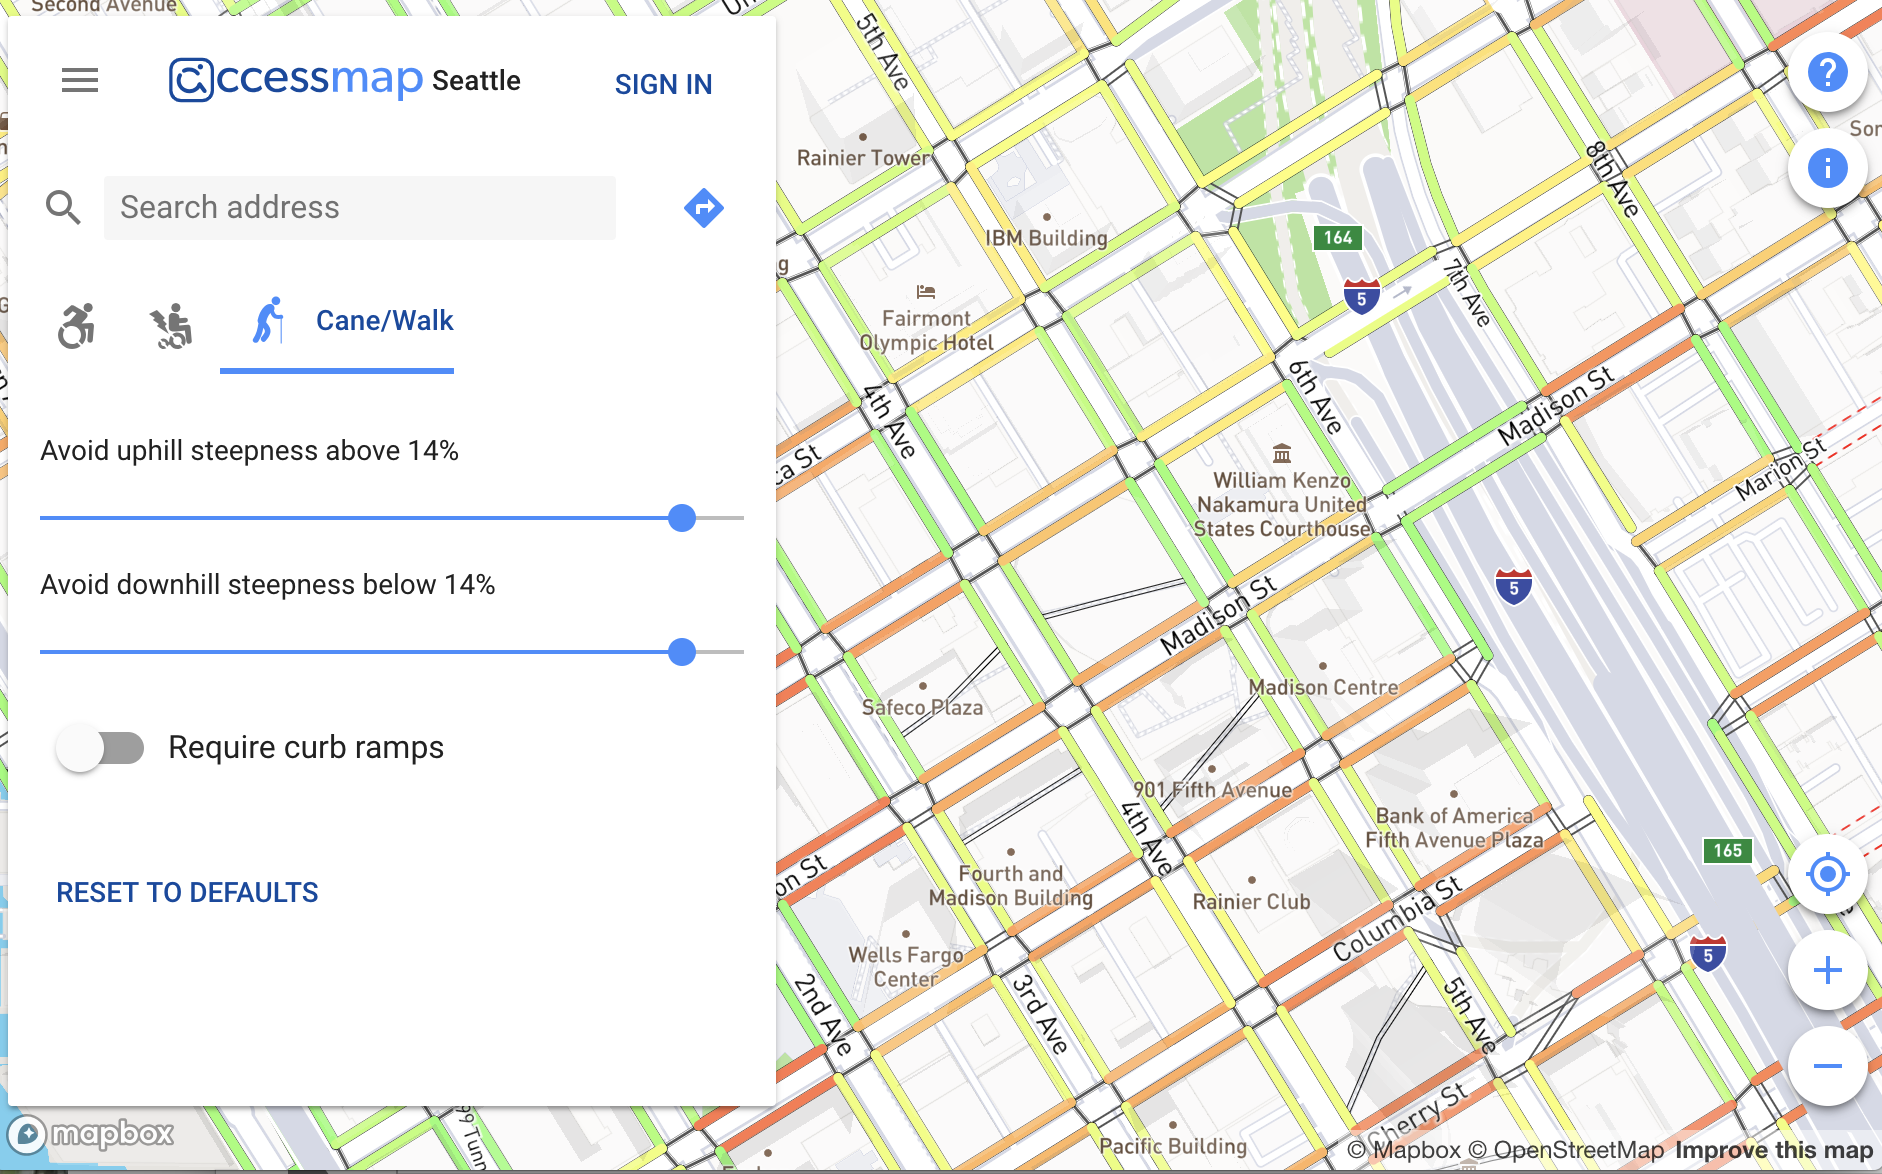
\includegraphics[width=5in]{pics/accessmap.png}
    \caption{AccessMap Screen Shot}
    \label{fig:accessmap}
\end{figure}

AccessMap currently can produce parametrically designed maps that always show the most up to data open data (derived from OpenSidewalks) about a region. 

\subsubsection{Proposed Development}

Operating hand-in-hand with AccessMap and OpenSidewalks (two projects discussed below), the goal of our work is to extend AccessMap to support users to automatically generate a custom 3D map model of any given area.  That model could then be printed at home, brought to a local library, or sent to a 3D printing service for relatively quick and inexpensive map production.  Beyond customizable map locations, ultimately the application would allow users to specify different scales and map features that are important to them.  

We will base our tactile design features on the comprehensive set of tactile map graphic symbols adopted by Braille Authority of North America (BANA) as created by (\cite{lobben2012tactile}, p. 107).% integrated into data driven design development tools and made available and consumable to landscape architects

%Anat: I commented this text out because I don't think it is product focused enough for NIDILLR's FIP in development. 
%The Tactile Maptile project designed the set of associated atomic symbols for that critical information.  Not only does this have implications for the map tiles specific to this project, but also more broadly works towards elevating pedestrian infrastructures in the context of our digital landscape.  This is important from a navigational perspective, but is also a reflection of the information designers, planners, and policy makers depend on to make significant decisions that affect our urban fabric.  Informed decisions based on incomplete data are not only difficult but also more prone to error and bias.  As we move rapidly towards sensor laced smart cities, it is critical these gaps be identified and understood in order to account for this influence on design and decision-making.  As such, this work is meant to take an accessible approach to data as it relates to pedestrian design and experience.

%Illustrative documentation of both the process and analysis that went into making these maps is directed more squarely at the design community. This project re-examines the pedestrian environment, with a focus on the specific needs of the low vision and blind communities. The goal of this work is to persuade designers to consider a broader spectrum of experience, and engage more critically in what it means to be designing inclusive cities.  

%This project is meant to bring attention to the deficiencies of the system currently place, in which accessibility checklists too often are accepted in lieu of truly inclusive design.  The straightforward approach is intended to remind designers that accessible design is good design, and if we want to build more equitable cities that means there is a huge spectrum of experiences we must first understand. 

\subsubsection{Validation}

\jm{ All studies need the following subsections to conform to the RFP:
\paragraph{Sample}
\paragraph{Environment}
\paragraph{Test Trials}
}

\ac{ needs writing


Our solution combines simple accessible interfaces with complex data integration and smart routing. To our users, the entire solution will be seamlessly presented in a workflow through which the travelers access a website, select the area of travel, the type of travel they wish to undertake in the area and travel preferences. The travelers are given the opportunity to verify the map location and features \textit{via} non-visual text-based exchange before printing the map.
% means what? A: means that in our UI pilot we found one of hardest things with building this UX/UI is ensuring that the tactile map model they got isn't of [Paris, Texas] when they actually meant [Paris, France]

The entire exchange is enabled and specifically designed for a portable 14-cell Braille-display. At the end, the traveler receives access to a downloadable 3D model file, access to an online URL where the model can be accessed for a specified duration, the option to have the model printed and sent to the user for a fee, and the option to subscribe to email alerts regarding any changes to the mapped region in the digital map repositories. 

}


\subsection{Automatically optimize map design based on specific needs (Mankoff\&Caspi-optimization.tex)}

\subsubsection{Background and State of the Art}

Route planning requires information that may be specific to the person creating a map. For example, Google Maps routes pedestrian directions from University Street Station on Second Avenue to Seattle City Hall on Fifth Avenue up Seneca Street, which has a steep 10 percent grade that is problematic for people in wheelchairs or with certain injuries or health conditions.
%SK:  how about older people?  That's not a "health condition" to me :).
%In contrast, AccessMap routes people two blocks north to Pike Street, which has a much gentler grade of less than 2 percent.
%For such people, it is important to ensure that a map clearly indicates slope. For those concerned about safety, however, it might be more important to show whether a guard rail is present near a particularly busy street, whether a sidewalk is wide or narrow near a busy street, or whether an alternative pedestrian route connects their sidewalk to a pedestrian footpath removed from the road. 
%For accessibility, 
users have varied needs.  A powered wheelchair user may need to know the location of curb ramps to navigate an intersection. A blind user may want to actively avoid certain types of curb ramps (such as those pointing to the center of an intersection). These different informational requirements present a particularly difficult situation to resolve without a detailed description of the available paths, how they are connected, and particular attributes (like curb ramps and their locations) \cite{bolten2017}. Furthermore, it is not possible to represent every possible piece of important information on any map. In particular, the amount of information that can be represented is further reduced in a tactile map. 
%SK:  Explain reason for preceding statement.

%SK.  Start discussion here.
\textit{Optimization} algorithms makes tactile maps accessible and actionable.  Here, we describe both: (1) optimizations that balance information richness with tactile usability, and (2) optimization cost functions that allow customization by Deaf-blind users of varied aspects of their travel experience.
%SK:  Now define optimization and what it does.

\jm{does this go in introduction instead?. also more about what optimization is/does A: I think that's where we were going before and it blew up the introduction. I think it's important to highlight here how optimization can make these maps actionable.}

\subsubsection{Previous Development: Optimization Approach}
Maps use many renditions to represent various forms of information. A  rendition could be a type of icon, or a colored line. Each rendition can represent only one class of information in a map. For example, a circular icon could note an accessible intersection, or a guide-dog friendly coffee shop, but it would be confusing if it represented both. Not all forms of information are compatible with all renditions. You cannot represent a road with just a circular icon. 
%The binary value stating if a a piece of information (a.k.a., a datum), $d$, is compatible with an rendition, $r$, is denoted $c_{rd} \in \{0,1\}$. If the datum is then assigned to a compatible rendition, this is denoted with the binary value: $x_{rd}\in \{0,1\}$

Our goal is to assign the most relevant pieces of information to the most useful renditions while maximizing the amount of information we present.  To do this, we need a model that describes what the most relevant information is.

%The zero-one linear program is formulated as follows:
%\begin{equation*}
%\textrm{ argMax }
%\sum_{i=1}^{|R|}
%\sum_{j=1}^{|D|}
%\alpha(r_i, d_j) x_{ij}
%\end{equation*}

%\begin{subnumcases}{
%\textrm{ s.t. } 
%}
%   \forall_{i \leq |R|} \forall_{j \leq |D|} r_{ij} x_{ij} \leq r_{ij} \label{data_rendition_compatability}\\
%   \forall_{i\leq|R|} \sum_{j\leq|D|} x_{ij} = 1 \label{rendition_Cap} \\
%\forall_{j\leq|D|} \sum_{i\leq|R|} x_{ij} \leq 1  \label{unary_data}\\
%\sum_{i\leq|R|} \sum_{j\leq|D|} x_{ij} = %\min(|R|, |D|) \label{complete_fill}
%\end{subnumcases}

%\item[Weighting Information-Rendition Pairings]
Specifically, when deciding how (or whether) to render a piece of information, we must consider three features with the acronym (CIA): the rendition's communicative ability (C), the data's importance (I), and the attentive cost (A).
%SK: Will readers know what "attentive cost" means? You use this interchangeably with "attention cost."  I changed all refs to the former for consistency.
We combine these by subtracting the attentive cost ($A$)  from the benefits ($C*I$): 
\begin{equation}
\label{eq::CIA}
\alpha(r_i, d_j) = C(r_i, d_j)*I(d_j)-A(r_i, d_j)
\end{equation}

\begin{description}
\item[Communicative Ability]
Communicative Ability, $C(r,d)$, is the measure of how well a rendition, $r$, communicates a specific type of information, $d$.
%A high level measure of this is already accounted for in the hard constraints of the linear program: if a rendition is incompatible (\ie incapable of communicating a class of information) constraint \ref{data_rendition_compatability} will not be met and the pairing will not be accepted. But our model must support more nuanced expressions of information communication. 
%For instance, there may be many types of renditions that label a coordinate on a map, but each are subject to certain limitations. 
For example, the number of parallel roads that can be represented in a space depends on the width of the lines representing the roads; denser road networks require thinner lines, while sparse networks could make use of more distinguishable, thicker lines. Further, certain attributes of a rendition may be more or less desirable to a specific user, such as the preference for braille or embossed text. 
%In our system, all renditions have a set of attributes, $a \in A_r$, (\eg uses braille, uses raised edges vs uses indented edges). Similarly, users profiles, $U$, and classes of information, $d$, have a set of preferred attributes, $\hat{A}_U,\hat{A}_d$ and weights on those preferred attributes $\beta_a$. 
More formally, the communicative ability of an information-rendition pairing is the weighted sum of the intersection of a rendition's attributes, an information class's preferred attributes, and a user's preferred attributes. 
\begin{equation}
\label{eq::communicability}
C(r,d,U) = \sum_{a\in A_r \cap \hat{A}_d}(\beta_a) +  \sum _{a\in A_r \cap \hat{A}_U}(\beta_a)
\end{equation}
%Attributes can be expressed in many ways, and determining the intersection of a rendition's attributes and preferred attributes is managed through a series of adapter interfaces. For instance, one interface is a Braille-compliant rendition, which requires the rendition to generate related text in braille. A user profile and information maintains a list of relevant adapters (\ie the preferred attributes) mapped to the preferential weight and any parameters of that preference. An example parameter is a preference for lines no thicker than 2 mm or no shorter than 1mm. These parameters are applied to the rendition through the adapter. 

\item[Information Importance]
%Information importance is the simplest measure of an Information-Rendition Pairing and it is central to the adaptive design paradigm our system represents. 
Users know what information is important to them. They know the accessibility features and challenges that affect them most, and what points of interest are most relevant to them. %For this measure, we simply 
Thus, we ask users to rank information. %, the higher the ranking, $I(d_j)$, of a class of information, the higher the weight. If the information is useless or irrelevant to the user the ranking is set to zero which intern makes the weight, $\alpha$, on all rendition pairings with this information zero or less, guaranteeing that the information will not be presented. For efficiency reasons, information classes that are marked as having no importance are excluded from linear program a priori. 
We can pre-populate this with default rankings based on a survey of typical user preferences. 

\item[Attentive Cost]
The attentive cost of a rendition measures how distracting it is to gather information from it. For example, if a user were using a rendition of a road network to navigate the map in search of a target, say their favorite coffee shop,  the longer it takes to find the target the more information they must keep track of (\textit{e.g.,} where they started, what turns they made, what landmarks they noticed). Tracking all of this information carries an attentive cost that would otherwise be spent on the primary search task.

A key problem here is that when the map is being constructed and the attentive cost weight is needed, we do not know what the user's target(s) will be, where they will start their search, or what other information is presented that may help or hinder the search task. To address this, we will use a Monte-Carlo simulation of user behavior based on our experimental work.\jm{megan: reference for monte carlo?} %The presentation of that information is, in fact, our goal. Given this level of uncertainty, we use a Monte-Carlo simulation to estimate the average \textit{time} it takes for the user to perform a search given a rendition-information pairing. The probability distribution used to generate this Monte-Carlo simulation is derived from a Markov-chain state model representing the actions a user can take when he or she encounters portions of a rendition. 
%\begin{figure}
%\label{fig::exampleStates}%
%	\begin{tikzpicture}
%        % Add the states
%        \node[state] at (0, 0) (o) {Off Road};
%        \node[state] at (4, 0) (r) {On Road};
%        \node[state] at (2, 4) (i) {Intersection};

%        \draw[every loop]
 %       	(i) edge[loop left] node {} (i)
%        	(i) edge[bend right=20] node %{} (r)
%            (r) edge[bend right=20] node {} (i)
%            (i) edge[bend right=20] node {} (o)
%            (o) edge[bend right=20] node {} (i)
%            (o) edge[loop left] node {} (o)
%            (r) edge[bend right=20] node {} (o)
%            (o) edge[bend right=20] node {} (r)
%            (r) edge[loop right=20] node {} (r);
%    \end{tikzpicture}
%\caption{Example of states of navigating a road network}
%\end{figure}
\end{description}

%Suppose that a user is navigating a rendition of a road network. There are three basic states of the action: (1) moving a finger along the road, (2) encountering an intersection of roads, and (3) moving a finger along the new road. Which particular state the user is in depends on the specific roads paired to the rendition, and their likelihood of moving from one state to another depends on both the particular road network (the information) and the rendition. For example, when the user encounters an intersection, he or she is very likely to continue onto a new road (\eg changing from the Intersection to On-Road state), but which road depends on many factors. Generally, the user is more likely to move in the same direction and increasingly less likely to turn all the way around. If the rendition presents very thin roads, the user is more likely to travel in a direction that they don't feel the roads any more, moving into the "Off-Road" state. We model the probability of this state change by selecting a random angle between $-\pi$ and $\pi$ from a normal distribution with a mean direction of 0 (no change in direction from the approaching road). If the user travels in that direction but could still feel a road (based on the width of the finger and thickness of the rendition), then the angle will be modified to continue along that road, otherwise they will move randomly in that general direction off-road until they find a new road to follow.  

%Each state change in the Markov-chain takes about step of one finger width, and we use a state change as a unit of time. For each simulation in the Monte-Carlo model, the user takes a "walk" across the map starting at a random point and moving towards a target. The starting points and targets are selected from a probability distribution where areas denser with information are more likely to be selected. The Markov-chain determines the walk that they take. We count the number of steps in the walk it takes to find the target given the rendition and information. The average number of steps over many models is our attention cost, meaning the more difficult (the longer it takes) it is to find information using a rendition-information pairing, the greater the attention cost and the poorer the pairing. 

%In terms of implementation, each rendition, $R$, has a set of states $S_R$. The probability of entering a state, $s_i\in S_R$, is dependent on the data, $D$, paired to $R$ and the state it is entering from, $s_{i-1}$: $P(s_i | D, s_{i-1})$, A walk over the map, $W$, starts from a starting point/state $s_1$ and we randomly change the state based on the probability distribution of all possible next-states. With each state we move the finger, $f$, a one finger width, $w_f$ in the direction dictated by the current state. The attention cost of a walk, $A(W)$, is the number of states need to get the point $f$ within $w_f$ of the target point $t$.The attention cost of a pairing, $A(R,D)$ is equal to the average attention cost of all of $N$ simulated walks.

%\begin{equation}
%W \subset S_R | s_1...s_{|W|}
%\end{equation}
%\begin{equation}
%A(W) = |W|
%\end{equation}
%\begin{equation}
%A(R,D) = \frac{\sum_{i=1...N} A(W_i)}{N}
%\end{equation}

\subsubsection{Proposed Development}

An optimization algorithm can use this information to decide on the optimal map. In optimization terms, $C*I-A$ is an \textit{objective function}, which can calculate a score for a possible map. Off-the-shelf algorithms can solve for the best solution (map in our case). For this problem, we can then  formulate the optimization as a zero-one linear program interpretation based on the Generalized Assignment Problem
\cite{kuhn1955hungarian}. 

\subsubsection{Validation}
\ac{JM: need your input here}
\ac{ make sure to include tests for both adequate balance for legibility and feature richness as well as tests for parametrization }

The following validation statements should be tested and hold true if the design goal for this development activity is met: 

The resulting tangible map depictions and choices will be valid.

\ac{this is just an example of a usability validation:}
When routing and choosing map features for no-vision pedestrians, the optimization algorithm favors streets with sidewalks and lower environmental stress (e.g., lower speed limits and traffic volume).

Here we describe our validation tests for both statements. The data elements and sources are referencing tests and data collection that will occur with our community partners. These data collection activities are described in later sections with greater detail.

\textbf{Validation Statement 1:
The resulting tangible map depictions and choices will be valid.}

\texttt{Performance Metrics:} 

\texttt{Data Elements \& Sources:}

\texttt{Analysis Procedure:}

\textbf{Validation Statement 2:
When routing and choosing map features for no-vision pedestrians, the optimization algorithm favors streets with sidewalks and lower environmental stress (e.g., lower speed limits and traffic volume).
}


\texttt{Performance Metrics:} 

\texttt{Data Elements \& Sources:}

\texttt{Analysis Procedure:}
\subsection{Enabling User to Produce Maps Themselves (Mankoff)}


\subsection{Conclusion}
needed?
%\section{Research Activities}
%Comment out if not a research proposal
%\subsection{Review of Current Literature}
\subsection{Research Hyotheses/Questions}
Be sure to argue that these are theoretically sound and based on current knowledge.
\subsection{Sample Justification}
Appropriate population; size; etc. to support proposed data analysis
\subsection{Data Collection Approach}
Appropriate to hypothesis/analysis
\subsection{Analysis Methods}
\subsection{Stakeholder Input}
How will individuals with disabilities and other key stakeholders provide input to shape the proposed research activities.
\subsection{Research Approach and Stages
     The applicant identifies and justifies the stage of research being proposed and the research methods associated with the stage.

\section{Evaluation Plan}
Plan for periodic assessment of progress toward implementing the plan of operation.

Assessment should be used to improve the performance of the project through the feedback generated.


\section{Staff}
\jen{Does the applicant encourage applications for employment from persons who are members of groups that have traditionally been underrepresented based on race, color, national origin, gender, age, or disability}

\jen{Are the proposed staff capable of doing the work.}

\subsectino{Anat Caspi}

\subsubsection{Capability in Project Domain}
\subsubsection{Encouraging Persons from Diverse Groups}

\subsection{Co-PI Mankoff}
P.I. Mankoff is the Richard E. Ladner Professor in the Allen School of Computer Science & Engineering 
at the University of Washington. She applies technologies such as data science and fabrication to 
improving inclusion in and accessibility of our digital future.  One of her primary application domains 
is revolutionizing the production and delivery of 3D printed assistive technology (\textit{e.g.,} \cite{Mankoff:2018:consumer,Hofmann:2016:HelpingHands,Chen:2016:Reprise}).

\subsubsection{Capability in Project Domain}
Jennifer has been a leader in the field of 3D printed assistive technology almost since its inception. Her work includes tool to facilitate the design of 3D printed devices \cite{Hofmann:2016:HelpingHands,Chen:2016:Reprise}; studies of how to integrate 3D printing into volunteer \cite{Parry-Hill:2017:Fabricators5} and clinical \cite{Hofmann:2016:Clinical} settings; and case studies highlighting how 3D printed assistive technologies might be received \cite{Hofmann:2016:HelpingHands}. Among her most relevant work are 
\begin{itemize}
    \item  A novel approach to creating tangible overlays for appliance screens that improve their accessibility \cite{Guo:2017:Facade}. The entire process can be accomplished by a blind person, from photographing the appliance (which is then analyzed by crowd workers) to ordering and attaching the overlay.  to two projects designed to improve the experience received her 
\item A study of the practices that visually impaired individuals use to learn about their environments which outlines requirements for independent spatial learning \cite{Banovic:2013:spatial}
\end{itemize}

Prof. Mankoff has been working in the field of accessibility since before she received her Ph.D.  at Georgia Tech. She teaches a quarterly accessibility seminar and has also taught longer courses on Assistive Technology and User Centered Research and Evaluation. She has also been chair of the SIGCHI Accessiblity community since 2014. She sits on the community council for the e-NABLE community \url{http://e-nable.org/}, a group of volunteers that work together to 3D print prosthetic hands world wide.

\subsubsection{Encouraging Persons from Diverse Groups}
Mankoff has mentored over 100
undergraduates. She estimates that 59\% are women (an under-represented category in computer science), 6\% latinx/African American, and 4\% disabled. Her group also includes (or has graduated) 14 Ph.D. students. Among these 14, 9 are female, 2 have a disability, and 1 is African American. 

These numbers reflect the fact that Prof. Mankoff regularly  leverages  historical knowledge of and connections to under
represented communities during the recruitment process to ensure that a representative group of students is considered for  positions. Similarly, her mentoring is designed to encourage and support students from varied backgrounds and ensure their success. 

\section{Resources}
Are the available resources (labs, etc) sufficient to do the work. 

Are the facilities accessible? What about online resources?
\section{Workplan}
The Work Plan should cover all three (3) years of the project period. The Work Plan should include a statement of the project's overall goal(s), anticipated outcome(s), and the major tasks that are proposed to achieve the goal and outcome(s). For each major task, the work plan should identify timeframes involved and the lead person responsible for the task.

NOTE : Applicants requesting funding for a multi-year grant program are REQUIRED to provide a Project Work Plan for EACH potential year of grant funding requested.
Goal:

Measurable Outcome(s):
* Time Frame (Start/End Dates by Month in Project Cycle)

% If you use beamer only pass "xcolor=table" option, i.e. \documentclass[xcolor=table]{beamer}
\begin{table}[h]
\resizebox{\textwidth}{!}{%
\begin{tabular}{@{}p{4cm}p{4cm}p{2cm}llllllllllll@{}}
\rowcolor[HTML]{333333} 
{\color[HTML]{FFFFFF} \textbf{Major Objectives}} & {\color[HTML]{FFFFFF} \textbf{Key Tasks}} & {\color[HTML]{FFFFFF} \textbf{Lead Person}} & {\color[HTML]{FFFFFF} \textbf{Q1}} & {\color[HTML]{FFFFFF} \textbf{Q2}} & {\color[HTML]{FFFFFF} \textbf{Q3}} & {\color[HTML]{FFFFFF} \textbf{Q4}} & {\color[HTML]{FFFFFF} \textbf{Q5}} & {\color[HTML]{FFFFFF} \textbf{Q6}} & {\color[HTML]{FFFFFF} \textbf{Q7}} & {\color[HTML]{FFFFFF} \textbf{Q8}} & {\color[HTML]{FFFFFF} \textbf{Q9}} & {\color[HTML]{FFFFFF} \textbf{Q10}} & {\color[HTML]{FFFFFF} \textbf{Q11}} & {\color[HTML]{FFFFFF} \textbf{Q12}} \\ 
1. &  &  &  &  &  &  &  &  &  &  &  &  &  &  \\
 &  &  &  &  &  &  &  &  &  &  &  &  &  &  \\
2. &  &  &  &  &  &  &  &  &  &  &  &  &  &  \\ \bottomrule
\end{tabular}%
}
\end{table}

\section{Related Work}
\ac{since we included related work in each development task, are we required to have this section?}
%\jen{From discussion with Harniss
Focus on the high level story about improving people’s lives
Significance section is really important}


%\subsection{Problem: What problem is being solved}
An ability to get from place to place, or \textit{navigate}, can allow individuals to take advantage of the  services and infrastructure embedded in the physical environment is critical to independent living. Indeed, a lack of mobility has been linked to social exclusion \cite{kenyon2002transport}.  Successful navigation can improve access to healthcare resources, education, financial resources (banks and other services) and participation in the workforce. Among these, participation in the workforce is one of the most important because of its ongoing impact on financial independence and social inclusion, and it lower for people with disabilities in general, and especially limited for Deaf individuals and Blind individuals \cite{zwerling2002workforce}.

Unfortunately,  navigational aids that meet the needs of  Deaf-Blind individuals are limited.

With more fundamentally visual personalized navigational apps coming to the market for people with disabilities, we must consider how experiences for people with both vision and hearing loss can be sensitively designed to provide comfortable, safe and delightful experiences mediating both destination-directed travel and exploration of the urban environment. 
Typical users are relegated to using Braille displays for Blind-Aware phone applications which have many drawbacks including sparse information that does not allow exploration of an area as opposed to route-following.
These solutions are typically expensive to produce and limited in their customizability (Rice, 2005). Despite indications that improving mass fabrication techniques for the production of tactile maps could be beneficial for people with both visual and hearing loss, this area remains relatively unexplored in contrast to the body of work on mobile navigation apps and other connected devices that serve as navigational aids.
Recent work has begun to explore the use of 3D printing to reduce cost, however other than our preliminary participant study (described below), we are not aware that these systems have been tested with Deaf-Blind individuals and lack customizability. 

Our solution is a system that can empower Deaf-Blind individuals to produce  customized, 3D printed tangible maps on their own. Our approach will maximize the integration of Deaf-Blind individuals into society by increasing their independence and their self-sufficiency. Our solution combines a method for generating custom maps with an accessible tool for generating these maps. We will iterative test our prototypes and process. In particular, in this proposal, we will demonstrate (1) The efficacy of our product in meeting the needs of Deaf-Blind individuals (2)  The iterative process that will allow us to define, test, and refine our product (3) our plan for assessing effectiveness and cost of our product. 

\subsection{Population: Who is being impacted}
\jm{xx text on deaf blind}

\subsection{Need: Our Community of Practice Experiences Daily Exclusion}

We conducted a  preliminary study with 27 Deaf-Blind individuals to assess need. We asked participants to explain how they travel and the issues most troublesome to them. 
Our study aimed to better understand how Deaf-blind people currently access community travel and 
accommodate inaccessibility in the built environment. In addition we were interested to know whether a tangible map we 3D printed for the area in which the participants met us added to their overall knowledge and confidence about their knowledge of that neighborhood.

We first asked the participants to meet us at the public library where the Deaf-Blind Service Center organizes community events. 
We observed their arrival to the library location. We also conducted semi-structured interviews with four individuals who are Deaf-blind their travel habits and strategies for using inaccessible built environments. 
We presented the participants a tactile map of the area in which we met them and asked participants to survey the tactile map. We asked them to find the location of the library in which we met which was signified by a \textit{landmark} tactile icon. We asked participants to explore the area and note any items, landmarks, street-names, buildings, bus stops or features that they understood to be in the area their hands were exploring. We observed the manner in which they explored the map and recorded their exploration via video. It should be noted that since individuals were conversing with us through an interpreted sign language, they would interrupt the exploration session to explain to us what they understood about the map.

We extracted the following key insights, which we will use to inform the design of this development project and we will also factor directly into the production of parsimonious yet useful tactile representations on the maps:

\begin{itemize}
  \item Participants felt that their city was becoming harder to access because the terrain is changing so fast. At first, they were surprised to learn via our tactile map about the new buildings and other changes to the environment. Some expressedly voiced frustrations, "...landmarks are disappearing! I thought this was there and now it is not. Now it is a big multi level building!" 

  \item All participants indicated they asked for help from a friend or stranger in their travel to the meeting location: frequently seeking help created a perceived social burden. Furthermore, participants worried that someone may not be available when they most needed it. Many indicated it is important for them to find alternate solutions that can increase the independence of the Deaf-blind in their daily lives.

  \item Labeling maps with Braille seemed a straightforward solution to us, but participants non-uniformly understood the abbreviations we used and some indicated discomfort with the 3D printed Braille that was produced via additive manufacturing, indicating it was too sharp to the touch.

  \item Participants found it difficult to do anything else when holding the map in one hand, tucking their cane under one arm and reading the tactile map with the other hand. In an actual travel scenario, such
difficulty might result in loss of orientation, thus interrupting
the travel task and potentially causing confusion and frustration.

  \item Providing tactile back with the right details, at the right density and frequency is crucial. For example, participants found it confusing when there was no tactile information when their finger was inside a large park. However, inserting tactile information in these situations brings up one of our main design challenges, e.g., the granularity and density of tactile presentation.
\end{itemize}

\ac{finish with a personal quote from Bruce}



jm{XX Anat, do you have any text on this?}

\subsection{Importance: How important is it to solve this problem }\jm{will generate a product or products (e.g., materials, devices, systems, methods, measures, techniques, tools, prototypes, processes, or intervention protocols) that can be used to maximize the full inclusion and integration into society, employment, independent living, family support, or economic and social self-sufficiency of individuals with disabilities, especially individuals with the most severe disabilities.}

\jm{XX Anat, do you have any existing text?}

xx something about how likely Deaf-Blind people are to be stuck at home/not educated/in the work force

xx something about general importance of independence, etc

??


This project presents an alternative approach to understanding the pedestrian experience. Challenging the existing primacy afforded to vision, this work takes a tactile approach. Physical abstractions are used as a means to guide people through the multi-sensory environments encountered everyday. Designed as tools that enhance spatial understanding for people within a large range of visual capacities, these maps consider circumstances that influence a full spectrum of experience. The maps produced confront gaps in the cartographic record as it pertains to inclusive design, and considers how that is manifest in the lived experience.

Impetus for research 

\ac{Mobility and orientation are biggest challenges for visually impaired people
GPS systems allow for verbal exchange of itineraries and navigation but do not allow for spatial understanding of environment. 
Maps are inherently visual and therefore inherently inaccessible
In addition to perpetuating challenges in mobility and navigation, results in social exclusion. There is a recognized need to design graphical material in an accessible way, but diversity of user group, available technologies and breadth of tasks create significant complexity 
}


%\SuspendCounters{page}
\renewcommand{\thepage}{}
\begin{appendices}
\SuspendCounters{page}
\section{Data Management Plan}
Nidler grants must comply with public access to publications requirement
++public access to data
+Data management Plan
++must submit one with proposal to meet public access requirement
++No strict answer to how to make data public, but all data must be public
++Does not count against 50 pages and not peer reviewed
++Should appear as an appendix
++What about Qualitative data?
+++No real answer other than "There are ways"
\jen{does not count toward page limit}

\subsection{Data to be collected}
\begin{itemize}
    \item Our data will include xxx software & map related data \jm{also meta data}
    \item Our  data will also include interview and 
survey data describing interactions with maps and analysis of artifacts from the field. Additional metadata will include coding schemes, memos, experiment protocols,  design recommendations and design ideas and scenarios of our proposed maps and map creation tools.
\end{itemize}

\subsection{How data will be organized, stored, and preserved}
\jm{Indication of whether the awardee will suhttps://www.overleaf.com/project/5c21099c86d1f25f54ca6267bmit the scientific data to ICPSR\footnote{applicants may seek technical assistance from the Interuniversity Consortium for Political and Social Research (ICPSR). ICPSR is the preferred data repository for archiving and sharing of scientific data generated under NIDILRR awards.}}

We will make the source code for our tools   available for public download  using an OSI-approved open source license. 

All human subjects will be anonymized and aggregated to maintain confidentiality 
and protect the privacy of subjects and industry partners. 
Key excerpts of anonymized primary data will be routinely shared 
in the context of publications of this research.  
Final coding schemes, design recommendations, and design prototypes will be shared in the context of publications of this work. Human subjects data that includes privileged and confidential information 
and will be kept secure in accordance with approved IRB protocols. \jm{Provide a plan to address the study participants’ consent process to enable the de- identified data to be shared broadly for future research.
} 
In the event that key data has not been published in formal venues within 
five years of the termination of this grant, 
all unpublished manuscripts will be made publicly available online.

\jen{If applicable, explain why data sharing, long-term preservation, and access cannot be justified.}

\jm{Indicate an estimated cost to implement the data management plan. This cost is allowable as part of the award’s direct costs.}
\section{Human Subjects}
%If you marked "Yes" for Item 3 on the Supplemental Information for SF 424, you must provide a human subjects "exempt research" or "nonexempt research" narrative. Insert the narrative(s) in the space provided. If you have multiple projects and need to provide more than one narrative, please indicate which project each set of responses addresses.

%\begin{itemize}
 %   \item Exempt Research Narrative. If you marked "Yes" for item 3a. and designated exemption number(s), provide the "exempt research" narrative. The narrative must contain sufficient information about the involvement of human subjects in the proposed research to allow a determination that the designated exemption(s) are appropriate. The narrative must be succinct. In addition, narratives are required for each participating partner if research is being conducted at other sites.
%    \item Nonexempt Research Narrative. If you marked "No" for item 3a., you must provide the "nonexempt research" narrative. The narrative must address the seven points. Although no specific page limitation applies to this section of the application, be succinct.
%\end{itemize}

%Human Subject Requirements for HHS grants. If your proposed project(s) involves research on human subjects, you must comply with the Department of Health and Human Services (DHHS)
%Regulations (Title 45 Code of Federal Regulations Part 46) regarding the protection of human research subjects, unless that research is exempt as specified in the regulation. All awardees and their performance sites engaged in research involving human subjects must have or obtain:
%(1) an assurance of compliance with the Regulations, and (2) initial and continuing approval of the research by an appropriately constituted and registered institutional review board. In
%order to obtain a Federal wide Assurance (FWA) of Protection for Human Subjects, the applicant may complete an on-line application at the Office for Human Research Protections (OHRP) website or write to the OHRP for an application. To obtain a FWA, contact OHRP at: http://www.hhs.gov/ohrp.

%For all proposed clinical trials, NIDILRR is requiring that applicants address the safety of human subjects participating in such trials or studies. This discussion must be identified in the application as a data and safety monitoring plan (Plan) and specifically address the safety of the participants and the validity and integrity of the data produced by the study. The Plan will be reviewed by NIDILRR staff prior to the award of the grant. Furthermore, a data and safety monitoring board (DSMB) is required for all multi-site clinical trials involving interventions that entail potential risk to participants. The data and safety monitoring plan must include a discussion of the DSMB if warranted by the proposed research activity. The Plan does not count against the page limitations described in this FOA and is not subject to the evaluation and scoring by the peer review panel.

%\subsection{Exempt Research Narrative}

%A. Exempt Research Narrative.
%If you marked “Yes” for item 3.b. and designated exemption numbers(s), attach the “exempt research” narrative to the Supplemental Information for the SF-424. The narrative must contain sufficient information about the involvement of human subjects in the proposed research to allow a determination by NIDILRR that the designated exemption(s) are appropriate. The narrative must be succinct.
%\subsection{ Nonexempt Research Narrative.}
%If you marked “No” for item 3.b. you must attach the “nonexempt research” narrative to the
%Supplemental Information for the SF-424. The narrative must address the following seven points. Although no specific page limitation applies to this section of the application, be succinct.
%\begin{description}

This proposal involves iterative design, including a number of studies that involve human subjects (specifically, Map Study 1 and 3; AccessMaps Study 1 and 2). 

\subsection{Human Subjects Involvement and Characteristics}

%Provide a detailed description of the proposed involvement of human subjects. Describe the characteristics of the subject population, including their anticipated number, age range, and health status. Identify the criteria for inclusion or exclusion of any subpopulation. Explain the rationale for the involvement of special classes of subjects, such as children, children with disabilities, adults with disabilities, persons with mental disabilities, pregnant women, prisoners, institutionalized individuals, or others who are likely to be vulnerable
Participants will include adults who are Blind (Map Study 1) and Deaf-blind (all other studies). Participants will be asked to take part in interviews, walkthroughs, and focus groups, paired with surveys, and questionnaires. In addition, participants will be asked to complete navigation tasks in field settings. 

\subsection{Sources of Materials}
%Identify the sources of research material obtained from individually identifiable living human subjects in the form of specimens, records, or data. Indicate whether the material or data will be obtained specifically for research purposes or whether use will be made of existing specimens, records, or data.

Materials will be collected during study sessions. These will include logs of behavior when using the online system, and recordings of interviews and study sessions. 

\subsection{Recruitment and Informed Consent}
%Describe plans for the recruitment of subjects and the consent procedures to be followed. Include the circumstances under which consent will be sought and obtained, who will seek it, the nature of the information to be provided to prospective subjects, and the method of documenting consent. State if the Institutional Review Board (IRB) has authorized a modification or waiver of the elements of consent or the requirement for documentation of consent.
Adults with visual or hearing impairments will be recruited.
We will recruit participants through community agencies in the Seattle Area such as the Lighthouse for the Blind and the Deaf Blind Service Center (DBSC). We’ll also partner with needs experts by asking them to share a description of our study by word of mouth and email. We will use snowball sampling to expand this pool. Informed consent will be a prerequisite to participation in all studies. 

\subsection{ Potential Risks}
%Describe potential risks (physical, psychological, social, legal, or other) and assess their likelihood and seriousness. Where appropriate, describe alternative treatments and procedures that might be advantageous to the subjects.

There are no direct benefits for participating in the study. Potential risks to participants include feeling uncomfortable discussing the character of their visual or hearing impairment and uncertainty about how to answer questions and finding the time it would take to participate in the study. However, the researchers will provide description of the study and explain that the participation is voluntary, participants can choose not to answer any or all questions, and can leave the study at any time. 

Although we will maintain confidentiality regarding participation and the qualitative data records will be de-identified, the participants will be unable to remain anonymous due to the nature of the interview, walkthrough and focus group methodologies.

Another risk is the inherent risk in navigating a city, on sidewalks shared by other pedestrians alongside roads with cars on them. Although this is a risk, it is no higher than the risk already faced by participants in their own everyday navigation activities. 

%(5) Protection Against Risk: Describe the procedures for protecting against or minimizing potential risks, including risks to confidentiality, and assess their likely effectiveness. Where
%appropriate, discuss provisions for ensuring necessary medical or professional intervention in the event of adverse effects to the subjects. Also, where appropriate, describe the provisions for monitoring the data collected to ensure the safety of the subjects.

\subsection{Importance of the Knowledge to be Gained}
%Discuss the importance of the knowledge gained or to be gained as a result of the proposed research. Discuss why the risks to subjects are reasonable in relation to the anticipated benefits to subjects and in relation to the importance of the knowledge that may reasonably be expected to result.

%\item[Collaborating Site(s)]: If research involving human subjects will take place at collaborating site(s) or other performance site(s), name the sites and briefly describe their involvement or role in the research.

%\end{description}

The knowledge gained through participation in our studies will help to improve the quality of our product, and ultimately to improve the navigation experience and opportunities available to Deaf-blind people. 


\section{Budget Narrative}
\label{budget}
See separate pdf (Budget.pdf)
\section{Letters of Commitment from Key Participating Organizations and Agencies}
Please include letters of commitment from Key Participation Organizations and Agencies after the Budget Narrative/Justification. Also please submit an appendix that lists
every collaborating organization and individual names in the application including
staff, consultants, contractors, and advisory board members. 
\section{OpenSidewalks Data Standard Description}

This Appendix includes an overview of features the OpenSidewalks data project collects pertinent to blind, low vision and Deaf-blind pedestrians. Surfaces are explored first, followed by topography, which is nearly as ubiquitous.  Street interfaces, while occupying less space in a pedestrian environment, arguably have the greatest impact on pedestrian safety and well-being and are the third feature set considered.
This section concludes with a brief overview of additional feature information, namely, transit stops, barriers, landmarks and points of interest; these topics, outside the scope of this work, nonetheless warrant further mapping and design research to enhance independence, mobility and safety for blind, low vision or Deaf-blind pedestrians.

\paragraph{Surfaces}
Surface materials have many distinct traits that are perceptible through the various senses.  Many significant non-visual characteristics affect any pedestrian’s experience, visually impaired or otherwise.
%SK: One could argue that smoothness and evenness (described below) are also visual characteristics. And why do you begin a discussion of surfaces by assuming cane use? Aren't wheelchairs also affected by smoothness and evenness? Should you discuss importance of smoothness and evenness in general before describing a specific use-case?
\begin{description}
    \item[Smoothness.]
Haptic canes make apparent even relatively minor changes in texture (like that found in stamped concrete).  Smoother surfaces require less effort to navigate with a cane.  
    \item[Evenness.]
Like smoothness, evenness can affect ease of navigation with a cane.  In addition, uneven surfaces have a higher potential to be a tripping hazard. 
    \item[Traction.]
Some surfaces are more prone to slipperiness than others. This can be a permanent feature of a material (e.g., a metal plate provides less traction than a gravel path) or a transient property, determined by seasonal (fallen leaves) or weather conditions (sleet).
    \item[Infiltration.] 
Without being able to identify potential water hazards in advance and determine an alternate route, the odds of inadvertently ending up with wet or damaged clothing increase.
    \item[Tactile Paving.] 
High-contrast, truncated dome tactile paving, most commonly found in the United States, is typically used for curb-ramps, stairs, and transit platforms. A variety of other textures -- including cones, bars and decorative paving -- can also be used for wayfinding or to alert pedestrians to a potential hazard.  
    \item[Width.] 
Wide (min 6’-12’) unobstructed paths are one of most straightforward ways to address access in a pedestrian environment (Goltsman and Iacofano 2007, Mitchell and Burton 2006).  They allow sufficient room for navigation with a haptic cane or assistive device and provide a buffer to adjacent traffic.  
%SK:  Not unless a physical buffer also exists, unless I misread the preceding sentence.
    
\end{description}


Ultimately, surface materials should be determined based on a path’s intended use.  To facilitate mobility, relatively smooth, unobstructed surfaces that are easy to navigate and provide adequate traction are best.  Textures can support spaces that are meant to do something more than simply move people through.   Material changes and textures can slow pedestrians down and inform them of transitions, hazards, or other circumstances that warrant attention.

\paragraph{Topography}
Grade change is experienced by everyone in even the flattest of cities on the flattest of blocks.  This work encourages designers to consider how topography affects the pedestrian experience at multiple scales.

\begin{description}
    \item[Macro.]
Despite the best efforts of some engineers (Klingle 2007), steep hills are often unavoidable elements of the urban fabric.  Significant topographical changes can enhance spatial understanding (Gardiner and Perkins 2005), but they nonetheless may pose a barrier to mobility. It is useful to consider ways in which this information might be mediated to the pedestrian's benefit.      
    \item[Transitional.]
Stairs and ramps help pedestrians negotiate site scale macro topography 
%SK:  huh?  What does "site scale macro topography mean"?
and provide common transitional elements to entrances for sites of interest.  Handrails and raised edges facilitate safe navigation.

    \item[Micro.]
Sidewalk cross-slope, curb heights, tree wells, planting beds, and other such features involve minor grade changes in urban environments.  While these may be empirically minor relative to a steep slope or staircase, they are no less significant when it comes to navigating as a pedestrian.  Edge detection, heading and orientation should be considered whenever a grade change is introduced.  If a non-intuitive change cannot be avoided, texture change or other signals can help to minimize conflict and injury.   

\end{description}


Topography often presents a challenge for designers, but accommodating grade change can also be seen as an opportunity to provide information to pedestrians as they move through space.  Edge detection is particularly important when designing with blind or low vision pedestrians in mind.  Potential signals that an edge is near may include the presence of railings, curbs and plantings, or a change in surface material. 

\paragraph{Street Interfaces}
Street interfaces are among the most dangerous spaces in the pedestrian built environment.  Advance knowledge facilitates safety, particularly for people who are blind or have low vision.
\begin{description}
    
\item[Curb Ramps.]
Well-designed curb ramps provide access to pedestrians that rely on assistive devices, but they also facilitate mobility for parents with strollers, cyclists, workers navigating with carts and countless other people with a vast range of circumstances and gear. Newly constructed curb ramps are typically outfitted with tactile pavement that alerts pedestrians to the transition into a vehicle-designated space.

\item[Directionality.]
Curb ramp directionality provides heading information to pedestrians as they exit a protected pedestrian area. As such, a curb ramp must guide the pedestrian into a safe crossing area.  Single curb ramps placed on a corner, or only on one edge of the sidewalk, risk directing pedestrians into traffic.  
%SK:  Why do "single curb ramps placed on a corner" direct pedestrians into traffic?  

\item[Shoring.]
Shoring, or a curb ramp’s raised edge, goes a step further than traditional curb ramps.  It provides an explicit safe heading, which offers navigational assistance to pedestrians using a white cane.  

\item[Crossings.]
For clarity and simplicity, crossing types have been grouped according to the following eight characteristics.  While these characteristics may exist independently, they are not mutually exclusive.  It is also important that these crossing features be considered in context with the street environment (e.g., number of traffic lanes, roundabouts, non-perpendicular intersections, etc.).  

\item[Unmarked Crossings.]
By far the most common crossing type is not marked at all. Any two sidewalk ends or corners separated by a street could be considered an unmarked crossing in certain locales.  Most intersections in residential and industrial neighborhoods fall into this category. Additionally, paint does not last forever: in many places throughout Seattle, marked crossings have all but disappeared as a result of weather and traffic.

\item[Marked Crossings.]
This term encompasses several crossing types that are characterized by a visual cue designed to inform both pedestrians and motorists that a pedestrian may be entering the street area.  Line styles can have different meanings depending on location; however, as a general rule, high contrast markings with greater surface area are easier to detect for both pedestrians and motorists. 

\item[Pedestrian Light Signals.]
This style of crossing signal provides pedestrians with a visual indicator of when it is safe to cross and is typically associated with a corresponding traffic light.  Some of these lights cycle automatically, while others require activation with a button.  In the City of Seattle, the buttons associated with this type of signal are typically rounded and require greater force to push than newer Accessible Pedestrian Signals (APS).

\item[Audible Signals.]
Audible pedestrian signals communicate the state of a crossing interval.  Modern signals are typically associated with a rapid ticking, or a verbal cue such as “walk sign is on” or “wait.”  Older “cuckoo-chirp” signals also fall into this category: a “cuckoo” sound is associated with safe north-south crossing, while “chirps” indicate an east-west pedestrian signal. Cuckoo-chirp style signals are no longer recommended since they tend to confuse pedestrians (Harkey et al. 2010).   

\item[Audio-Tactile (Vibrating) Signals.]
Modern accessible pedestrian signals include a haptic indicator embedded in the crossing signal's push button.  This type of signal is particularly useful for the deaf-blind community, but it also provides a clearer indication of what direction is safe to cross for pedestrians who are blind or have low vision relative to audible overhead signals.  In Seattle, audio-tactile APS systems are typically associated with flat push buttons that require less force to activate than the older systems.

\item[Raised Pedestrian (Tabled) Crossings.]
This increasingly popular type of crosswalk is kept at grade with the sidewalk, encouraging cars to slow down and giving pedestrians priority.  However, in the absence of the grade change that typically signals to pedestrians that they are entering a car-dominant area, it is important to provide a tactile cue through a surface change or warning strips to pedestrians who are blind or have low vision. 

\item[Traffic (Refuge) Islands.]
These painted or raised areas can be located between large traffic lanes, or at the junction of multiple streets intersecting in a non-perpendicular fashion.  Ideally, they  are accompanied by additional pedestrian safety features such as: high contrast tactile paving, shoring edges to provide heading, signage and pedestrian signals.

\item[Pedestrian Bridges and Tunnels.]
Pedestrian bridges and tunnels mitigate traffic conflicts by routing pedestrians on a separate plane or z-level.  To promote accessibility, these features must address the needs of those using assistive devices and make clear both their presence and the locations of their entrances and exits, if separate from the path itself.
\end{description}

A pedestrian’s experience of any street interface depends significantly on the vehicular environment.  Tactile map design should consider ways to facilitate safety and mobility from the pedestrian's perspective, and especially consider the motorist's ability to see a vision-limited traveler. Traffic-calming strategies, such as enlarged corner bulbs, are preferable when optimizing a route for a blind individual. 
%SK:  Does reader know what "corner bulbs" are?


\paragraph{Transit} 
Public transit provides access to the city for millions of riders each year.  Predictably, far side bus stops are preferred in Seattle (Seattle 2005). 
%SK:  What are "far side bus stops"?  I'm thinking a small Glossary would be a big asset for this (and future) proposals.
However, these are not ubiquitous. Being aware of alternative options helps designers better accommodate these inconsistencies in the urban fabric and facilitate understanding for riders. With more information made available, travelers are more likely to attempt unfamiliar trips on public transportation (Campbell et al. 2014).  

Given the importance of transit information, the maps produced 
%SK:  what 'maps produced"? By whom? The "current DOT transit maps present..."?
represent transit stop locations; however, spatial constraints restricted the granularity of data that could be associated with these stops. Ideally, critical information would be available through a linked app that could read bus numbers and location details to the user.  At the very least, this more detailed information should be available at bus stops.  Unfortunately, Braille is notably absent from the vast majority of informational signage at transit stations. 

\paragraph{Barriers, Landmarks and Points of Interest}
Barriers (construction sites, low hanging branches, sandwich boards, pavement cracks…), landmarks (fountains, play fields, churches…) and points of interest (retail, food, services...) are additional categories that should be considered in relation to wayfinding, mobility and the pedestrian experience.  The vast range of potential features, as well as their subjective nature, precluded them from an in-depth investigation in this study.  However, there is precedent and opportunity to explore these features in future work.   


\label{sec:standarddata}
\end{appendices}

\pagebreak

\bibliographystyle{apalike}
\bibliography{bibliography}
%\printbibliography


\end{document}
